\chapter{Proyecto de Ruby on Rails}

\section{Fase de análisis}

\subsection{Requisitos funcionales}

\begin{enumerate}[label=\textbf{RF-\arabic*}]
	\item
		\textbf{Registro de jugador}
		\begin{itemize}
			\item
				\textbf{Descripción:}
				Un jugador debe poder registrarse mediante un formulario.
			\item
				\textbf{Entrada:}
				Correo electrónico y contraseña.
			\item
				\textbf{Procesamiento:}
				Los datos del jugador se introducen en la base de datos mediante una consulta de inserción.
			\item
				\textbf{Salida:}
				El jugador se encuentra registrado en la base de datos e inicia sesión automáticamente.
		\end{itemize}
		\begin{enumerate}[label=\textbf{RF-1.\arabic*}]
			\item
				\textbf{Inicio de sesión}
				\begin{itemize}
					\item
						\textbf{Descripción:}
						Un jugador registrado debe poder iniciar sesión.
					\item
						\textbf{Entrada:}
						Correo electrónico y contraseña.
					\item
						\textbf{Procesamiento:}
						Los datos del jugador se comprueban en la base de datos mediante una consulta y se determina si son correctos, en cuyo caso se inicia su sesión.
					\item
						\textbf{Salida:}
						El jugador queda con la sesión iniciada si los datos son correctos o recibe un error en caso contrario.
				\end{itemize}
			\item
				\textbf{Cierre de sesión}
				\begin{itemize}
					\item
						\textbf{Descripción:}
						Un jugador con sesión iniciada debe poder terminarla.
					\item
						\textbf{Entrada:}
						Petición de cierre de sesión.
					\item
						\textbf{Procesamiento:}
						Se guardan los datos del jugador pendientes de escritura y se destruye su sesión.
					\item
						\textbf{Salida:}
						La sesión del jugador queda cerrada y debe volver a iniciarla para interactuar con el sistema.
				\end{itemize}
		\end{enumerate}
	\item
		\textbf{Estado de juego persistente}
		\begin{itemize}
			\item
				\textbf{Descripción:}
				El servidor almacena el estado del juego de los jugadores.
			\item
				\textbf{Entrada:}
				Estado actual del juego de uno de los jugadores.
			\item
				\textbf{Procesamiento:}
				Se realizan consultas periódicas a la base de datos que almacenan el estado del juego.
			\item
				\textbf{Salida:}
				El estado del juego del jugador queda registrado en la base de datos.
		\end{itemize}
	\item
		\textbf{Experiencia acumulada}
		\begin{itemize}
			\item
				\textbf{Descripción:}
				Las acciones del juego añaden puntos de experiencia al jugador.
			\item
				\textbf{Entrada:}
				Interacción con el juego.
			\item
				\textbf{Procesamiento:}
				Se añade una cantidad de experiencia al perfil del jugador.
			\item
				\textbf{Salida:}
				El jugador tiene más puntos de experiencia.
		\end{itemize}
	\item
		\textbf{Nivel del jugador}
		\begin{itemize}
			\item
				\textbf{Descripción:}
				El jugador tiene un nivel calculado por su experiencia.
			\item
				\textbf{Entrada:}
				Experiencia acumulada por el jugador.
			\item
				\textbf{Procesamiento:}
				Se calcula el nivel del jugador mediante una fórmula matemática.
			\item
				\textbf{Salida:}
				El nivel total del jugador.
		\end{itemize}
	\item
		\textbf{\textit{wiki}}
		\begin{itemize}
			\item
				\textbf{Descripción:}
				Existe una \textit{wiki} en la que consultar el manual de jugador del juego.
			\item
				\textbf{Entrada:}
				Petición de búsqueda de una página de la \textit{wiki}.
			\item
				\textbf{Procesamiento:}
				Se realiza una consulta a la base de datos de selección de la página requerida por el jugador.
			\item
				\textbf{Salida:}
				Páginas coincidentes.
		\end{itemize}
	\item
		\textbf{Perfil de otros jugadores}
		\begin{itemize}
			\item
				\textbf{Descripción:}
				Se puede consultar el perfil de los diferentes jugadores
			\item
				\textbf{Entrada:}
				Identificador del usuario a consultar.
			\item
				\textbf{Procesamiento:}
				Se realiza una consulta de selección del usuario requerido por el jugador.
			\item
				\textbf{Salida:}
				Información del usuario consultado.
		\end{itemize}
	\item
		\textbf{\textit{Ranking} de jugadores}
		\begin{itemize}
			\item
				\textbf{Descripción:}
				Se puede consultar un \textit{ranking} de los jugadores con más experiencia.
			\item
				\textbf{Entrada:}
				Acceso al \textit{ranking}.
			\item
				\textbf{Procesamiento:}
				Se buscan los 25 jugadores con más experiencia.
			\item
				\textbf{Salida:}
				Información de los 25 jugadores con más experiencia.
		\end{itemize}
\end{enumerate}

\subsection{Requisitos no funcionales}

\begin{itemize}
	\item
		Los jugadores que quieran interactuar con el sistema deben estar registrados con su correo electrónico y haber iniciado sesión previamente.
	\item
		La \textit{wiki} debe ser accesible desde la página web para que los jugadores puedan consultarla sin interrumpir su experiencia.
	\item
		El código debe ser libre y estar disponible para todo el mundo sin trabas bajo la licencia GPL-3.0.
	\item
		El acceso a la base de datos debe ser eficiente, de forma que el jugador no experimente retardos en las operaciones que realiza sobre el sistema.
	\item
		El acceso a la base de datos debe ser seguro para garantizar que no exista la posibilidad de inyectar código que pueda vulnerar la privacidad del resto de jugadores.
	\item
		La página web debe ser accesible según el estándar W3C\@.
		\begin{itemize}
			\item
				Las fuentes utilizadas en la web deben ser fácilmente legibles en pantallas de alta y baja resolución, de forma que el jugador no tenga problemas para navegar por el sitio.
			\item
				La página web debe ser ligera para todos los dispositivos para que cualquier jugador pueda entrar en ella sin problemas.
		\end{itemize}
\end{itemize}

\subsection{Partes interesadas y preocupaciones}

\begin{itemize}
	\item
		\textbf{Usuarios del juego:}
		Quieren disfrutar de la experiencia que ofrecemos.
	\item
		\textbf{Desarrolladores:}
		Quieren aprobar la asignatura.
	\item
		\textbf{Comunidad \textit{open source}:}
		Quieren aprender sobre cómo hemos trabajado y expandir las funcionalidades del sistema.
	\item
		\textbf{Inversores:}
		Ven una posibilidad de introducir elementos en el juego que les genere beneficio.
\end{itemize}

\subsection{Diagrama arquitectónico}

\begin{figure}[!ht]
\begin{center}
	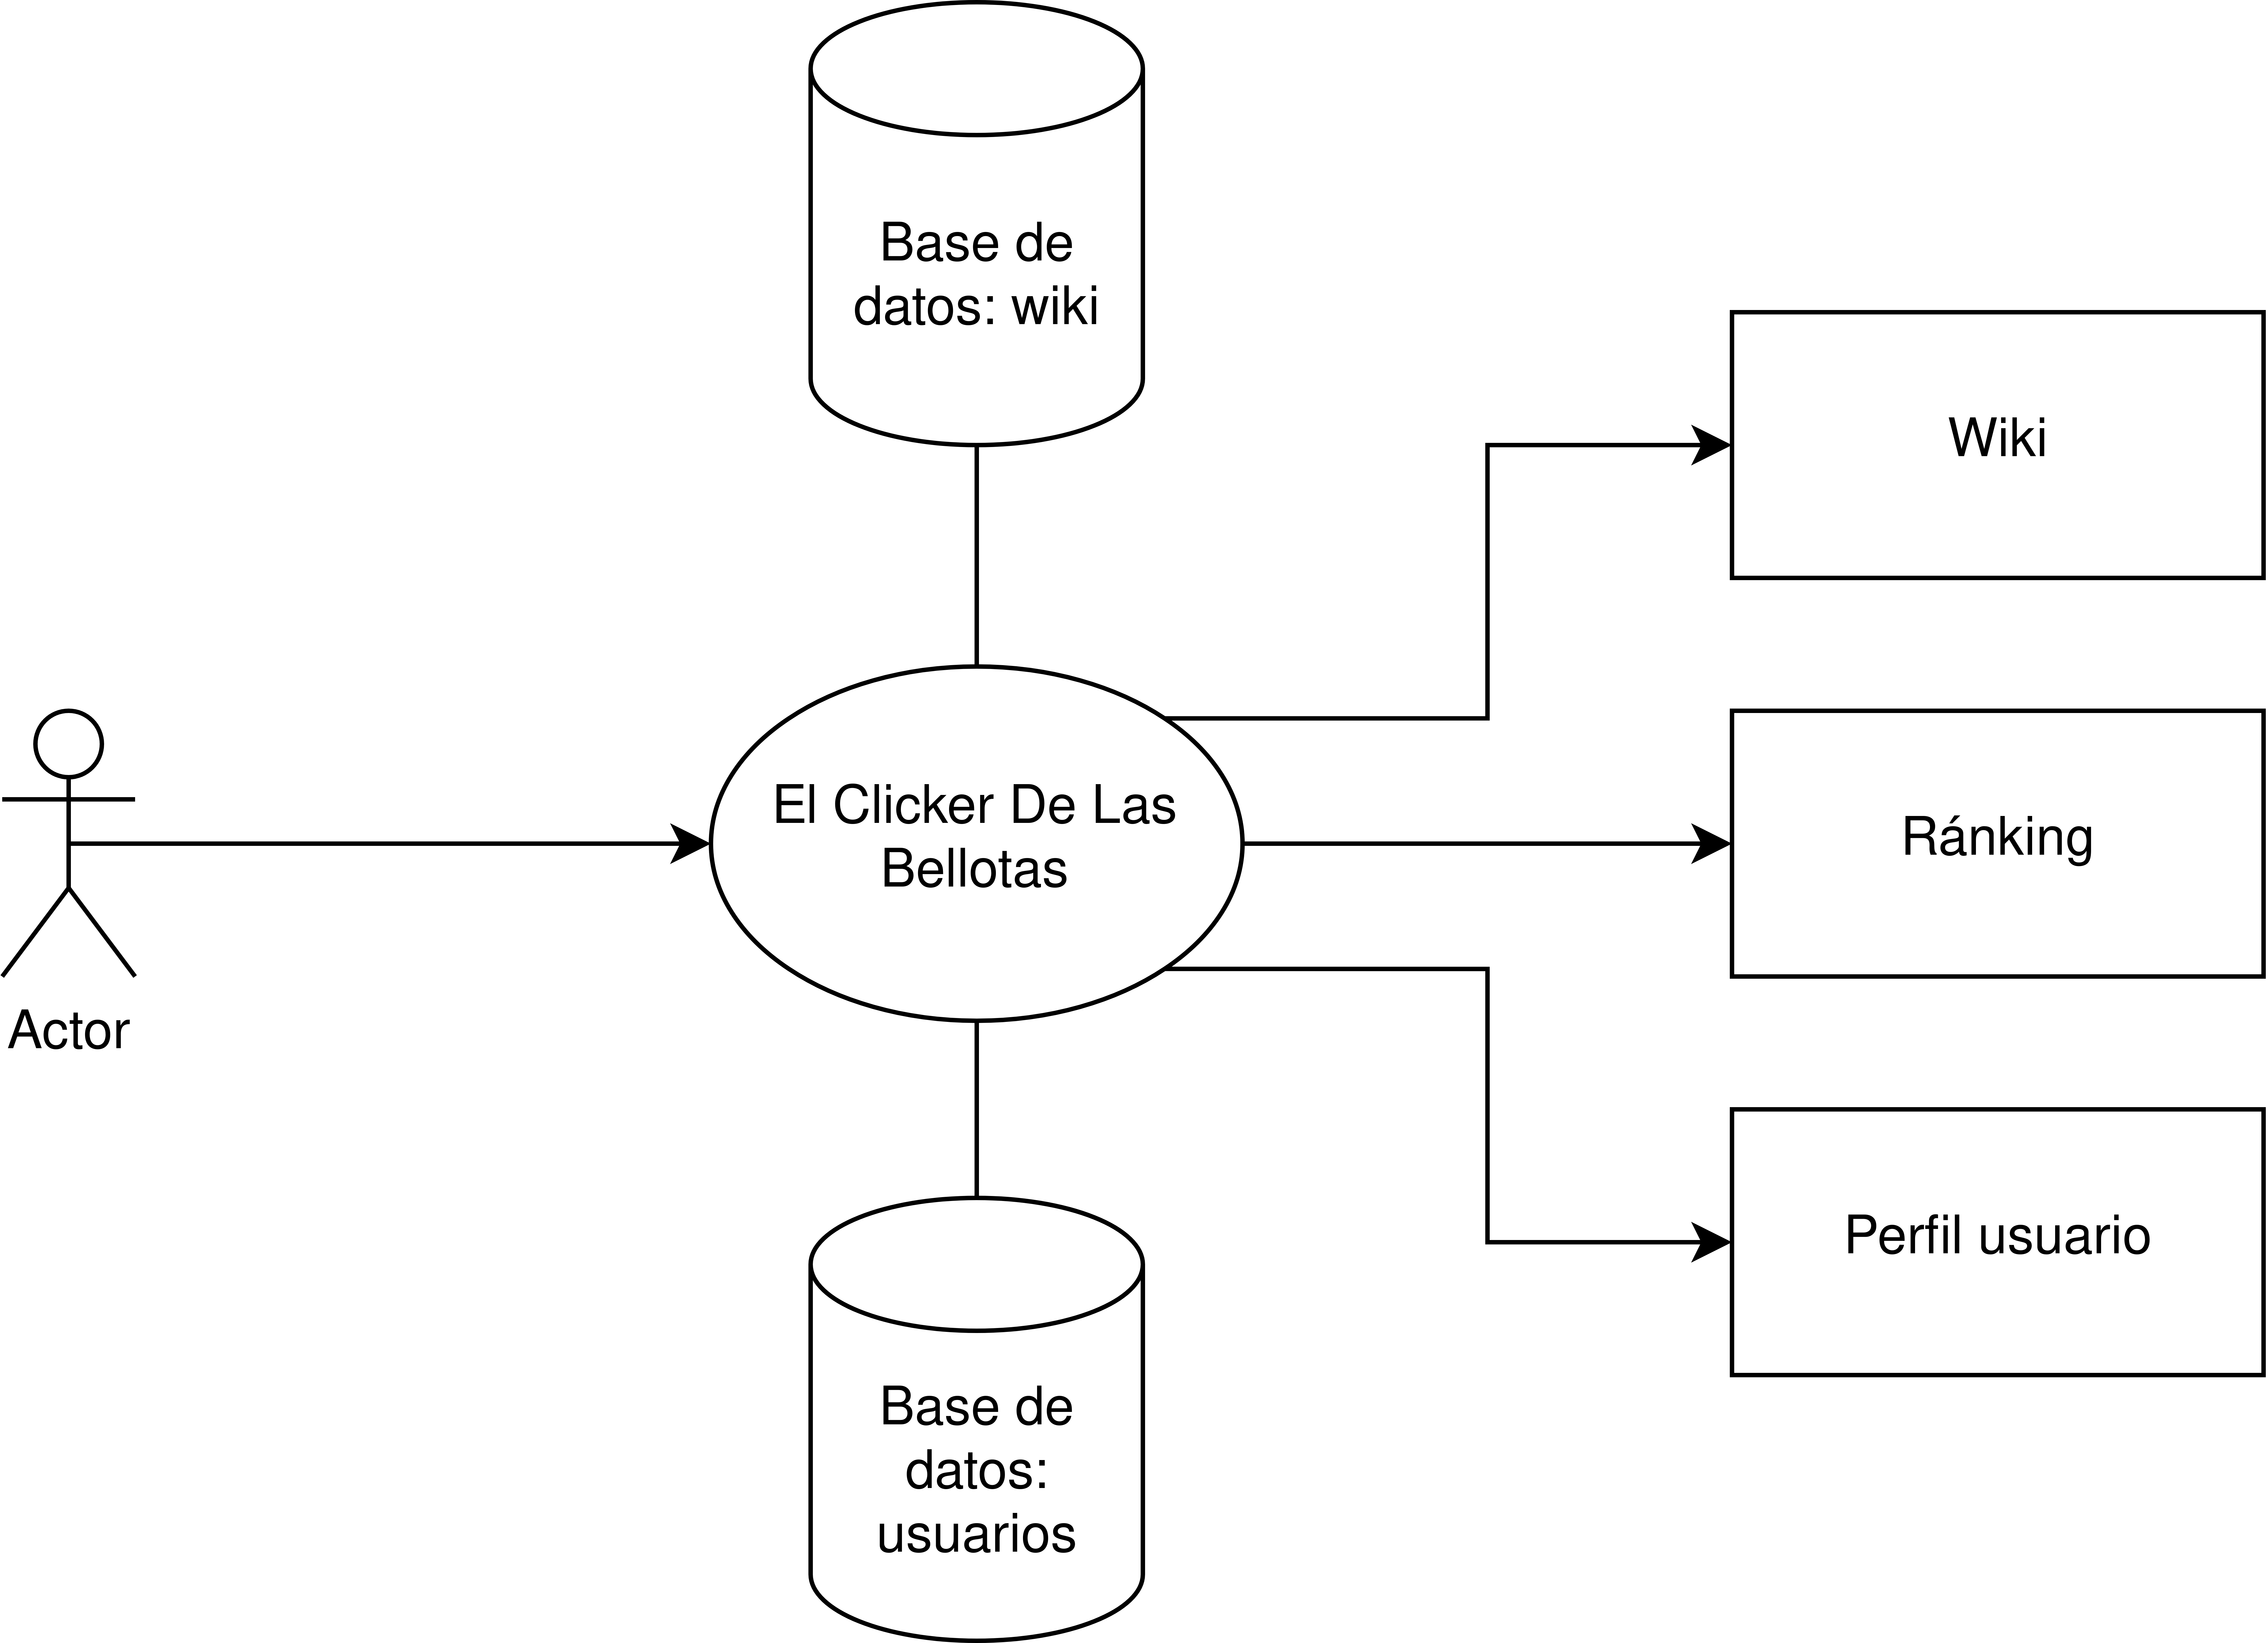
\includegraphics[scale=0.04]{Diagrama de contexto}
\end{center}
\caption{Diagrama de contexto de nuestra aplicación}
\end{figure}

\subsection{Criterios de calidad}

\begin{itemize}
	\item
		\textbf{Seguridad:}
		Los datos de los jugadores deben estar protegidos contra ataques que violen su privacidad, como inyecciones de código y accesos no autorizados a los datos.
	\item
		\textbf{Fiabilidad:}
		El sistema debe estar siempre en funcionamiento y los accesos a la base de datos deben ser correctos.
		En caso de fallo, se garantiza la menor pérdida de información posible debido a la periodicidad de la escritura del progreso de los jugadores.
	\item
		\textbf{Mantenibilidad:}
		Todo el código y el acceso al sistema debe ser libre, de forma que las modificaciones puedan ser hechas por la comunidad.
	\item
		\textbf{Completitud:}
		El sistema debe cumplir en todo momento con las indiciaciones de las ESRB y PEGI\@.
\end{itemize}
